\begin{definition} Схемой из функциональных элементов называется ориентированный граф без циклов, в котором каждая вершина помечена одной из пяти меток: in, out, $\neg$, $\wedge$, $\vee$. При этом соблюдаются следующие условия на входящие и исходящие степени: \end{definition}
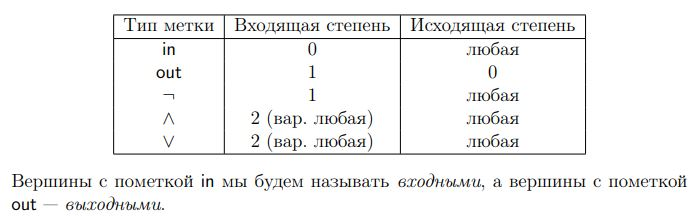
\includegraphics[]{images/scheme.JPG}

\begin{definition} Высотой вершины будем называть длину самого длинного
пути от некоторой входной вершины до данной. Поскольку в графе нет циклов,
этот максимум корректно определён. \end{definition}

\begin{definition} Размером схемы называется количество вершин в графе.
Глубиной схемы называется максимальная высота вершины. \end{definition}

\begin{definition} $\ppoly$~---  класс языков, распознаваемых схемами полиномиального размера (не глубины, а именно число элементов). \end{definition}

\begin{definition} Прямолинейная программа~--- последовательность, состоящая из набора изначальных переменных и набора присваиваний, справа от которых либо отрицание, либо конъюнкция, либо дизъюнкция, а слева либо уже полученная ранее в ходе присваиваний, либо одна из исходных. Некоторые переменные помечены как выходные. \end{definition}

\begin{statement} Для каждой схемы есть прямолинейная программа, вычисляющая ее, и наоборот. \end{statement}

\begin{proof} По схеме построить программу легко. Всем входным вершинам сопоставляем набор входных переменных, а потом поуровнево пишем присваивания. По программе тоже линейно строим дерево ее разбора (точнее DAG) и получаем схему. Более того, можно сначала построить схему в виде дерева, используя переменные несколько раз, а потом одинаковые вершины отождествить.

\end{proof}

\begin{definition} Классом $\adtime{t(n)}{\alpha(n)}$ называется класс языков $A$ таких, что существует МТ $M$ и последовательность подсказок $\alpha_n$ длины $\mathcal{O}(\alpha(n))$ таких, что $M(x, \alpha_{|x|}) = 1 \iff x \in A$, при этом время работы составит $\mathcal{O}(t(n))$. \end{definition}

\begin{statement} $\ppoly = \bigcup\limits_{c, d = 1}^\infty \adtime{n^c}{n^d}$. \end{statement}

\begin{proof} Пусть $A \in \ppoly$, тогда передадим в качестве подсказки схему под слово длины $|x|$, распознающую слово. Она имеет размер poly$(|x|)$, а МТ просто исполнит эту схему за линейное от размера схемы (или полиномиальное от $|x|$) время.

В обратную сторону. Переделаем машину в схему (аналогично теореме Кука-Левина), у которой будет две группы входов: для $\alpha$ и для $x$. Так как $\alpha$ это полином от $|x|$, получим, что схема сама по себе полиномиального размера. В итоге схема будет иметь вид входа $x$ и зафиксированной подсказки в виде второго аргумента (она одна и та же для всех слов одной и той же длины).

\end{proof}